\section{Experimental Results}
\label{sec:evaluation}
The following results combine retained completed controls with the newer
exploratory laptop pilots. Tables identify their execution scope. The
cost-aware text rerun and native rank ablations are reported without
assigning them missing paired timings or server-level performance claims.

\subsection{RQ1: Contribution of the Certificate Components}
\label{sec:ccd-rq1}
\subsubsection{Exact groups and switching information}
The saved 19-update development workload provides a direct mechanism check.
The groupwise moments-only upper bound certifies two improvements, whereas
the complete switching certificate resolves all nineteen. The additional
seventeen improvements cannot be concluded from that moments-only bound.
This comparison recomputes bounds on a retained completed workload; it is
not a new timing experiment for moments-only.

The completed larger Fashion control in Table~\ref{tab:ccd-archive} adds a
different case: three naturally worsening updates with nonzero switching.
Both compact bases certify all three. The moments-only control requires
Full on every update and takes 134.413 minutes, including its unsuccessful
work and exact fallback. The centroid certificate takes 42.534 minutes
against 101.575 for Full. These observations support the role of switching
information beyond a one-sided improvement test.
\begin{table}[tbp]
\centering
\small
\caption{Archived completed Fashion control, $n=1024$, $k=5$, seed 173 and reference step 8. Frozen models are supplied and eight workers are used. Times are minutes, including preparation, proof work, replay and paid fallback. This is a separate workload from the new seed 521 pilots.}
\label{tab:ccd-archive}
\begin{adjustbox}{max width=\columnwidth}
\begin{tabular}{lrrrrr}
\toprule
Method & Min. & Full min. & Ratio & Cov. & FB\\
\midrule
Centroid & 42.534 & 101.575 & 2.388 & 3/3 & 0\\
Moments-only & 134.413 & 101.575 & 0.756 & 0/3 & 3\\
PCA & 44.156 & 101.575 & 2.300 & 3/3 & 0\\
\bottomrule
\end{tabular}
\end{adjustbox}
\end{table}


\subsubsection{Basis rank and refinement budget}
The new native ablation fixes prediction rank 63 and varies certificate rank
and correction cap. At $n=128$, rank 4 and cap 16, the centroid-informed basis
resolves six of eight Fashion updates, while PCA resolves one. At ranks 39,
63 and 79 both resolve all eight. Table~\ref{tab:ccd-ranks} also records the
number of corrected rows. This low-rank contrast is evidence about the
geometry of the envelopes, not a measured proof-speed advantage.
\begin{table}[tbp]
\centering
\small
\caption{Native-only Fashion ablation; prediction rank remains 63 and the correction cap is 16. Cov. is conclusive update coverage and Rows is the total corrected-row count across eight requests. No proving time is inferred.}
\label{tab:ccd-ranks}
\begin{adjustbox}{max width=\columnwidth}
\begin{tabular}{rrrrrr}
\toprule
$n$ & $s$ & Cent. cov. & Rows & PCA cov. & Rows\\
\midrule
32 & 4 & 8/8 & 28 & 8/8 & 80\\
32 & 39 & 8/8 & 7 & 8/8 & 9\\
32 & 63 & 8/8 & 5 & 8/8 & 5\\
32 & 79 & 8/8 & 4 & 8/8 & 5\\
128 & 4 & 6/8 & 72 & 1/8 & 112\\
128 & 39 & 8/8 & 1 & 8/8 & 1\\
128 & 63 & 8/8 & 0 & 8/8 & 0\\
128 & 79 & 8/8 & 0 & 8/8 & 0\\
\bottomrule
\end{tabular}
\end{adjustbox}
\end{table}


\begin{figure*}[tbp]
\centering
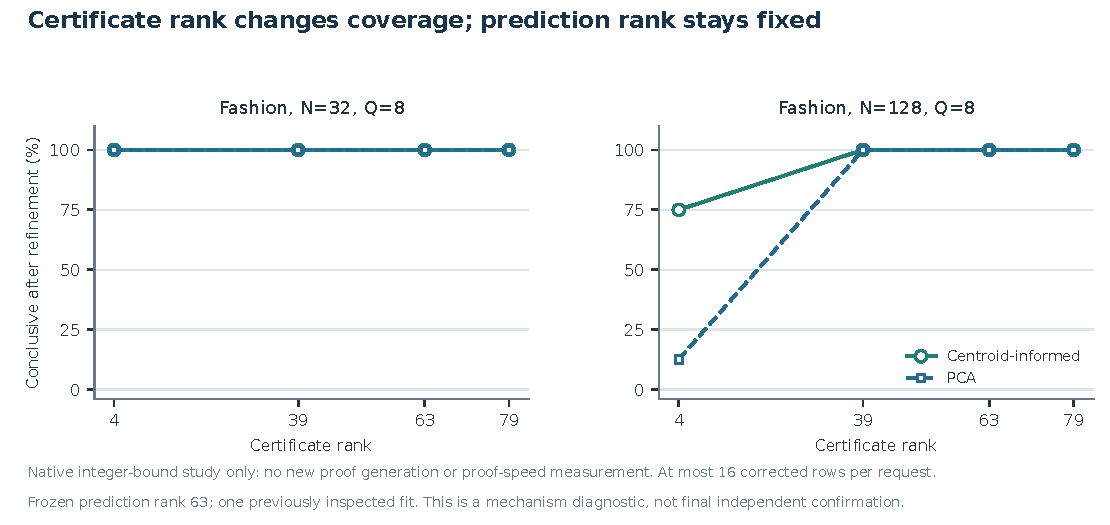
\includegraphics[width=.96\textwidth]{paper_results/ccd_pilot_20261029/figures/07_rank_coverage_native_only.pdf}
\caption{Native-only certificate-rank ablation on the retained Fashion fit.
Prediction remains rank 63. Coverage is measured after at most 16 corrections
per request. Coincident curves at higher ranks indicate equal coverage;
the plot contains no proof-generation timings or independent-fit interval.}
\label{fig:ccd-rank-coverage}
\end{figure*}

At the deployed rank 79 profile, the eight-request Fashion proof pilot
requires four correction proofs with the centroid-informed basis and five
with PCA. Both resolve all requests and have 100\% assignment agreement on
that small catalog. On text, both resolve only two of eight before fallback,
and both have 95.703\% assignment agreement. The larger native study retained
in Appendix~\ref{app:ccd-evidence} supplies additional application checks;
it does not make the single-fit low-rank contrast a general ranking.

\paragraph{Answer to RQ1}
Authenticated exact groups make the assigned contribution exact, while
switching information and verified corrections can resolve updates left
open by group moments. Basis choice affects interval quality, especially
at low certificate rank. The present evidence does not establish a
consistent runtime advantage over equal-rank PCA at the default profile.

\subsection{RQ2: Preparation, Request Cost and Reuse}
\label{sec:ccd-rq2}
\subsubsection{Cold campaign comparisons}
Table~\ref{tab:ccd-cold} reports the earlier seed-521 cold comparisons. On
Fashion with $n=32$ and eight requests, the centroid certificate takes 9.867 minutes,
compared with 13.093 for Full and 7.430 for the ZKML adapter. It is cheaper
than the internal Full implementation but more expensive than the adapter.
PCA is close at 9.992 minutes. Thus the eight-request result does not support
a single ranking across all implemented systems.
\begin{table*}[tbp]
\centering
\small
\caption{Completed exploratory cold campaign comparisons. Times are minutes and include the preparation, generation, replay and paid fallback retained by each campaign. Q8 totals retain recorded fitting; the Q16 follow-up supplies frozen fitted inputs. Coverage and FB concern the centroid certificate before and after fallback. The missing PCA N128 entry was interrupted by a host-memory guard.}
\label{tab:ccd-cold}
\begin{adjustbox}{max width=\textwidth}
\begin{tabular*}{.98\textwidth}{@{\extracolsep{\fill}}lrrrrrrrr@{}}
\toprule
Data & $n$ & $Q$ & Full & ZKML-ad. & Centroid & PCA & Cov. & FB\\
\midrule
Fashion & 32 & 8 & 13.093 & 7.430 & 9.867 & 9.992 & 8/8 & 0\\
Text & 32 & 8 & 5.964 & 3.751 & 16.090 & 16.186 & 2/8 & 6\\
Fashion & 128 & 4 & 22.838 & 15.525 & 12.467 & -- & 4/4 & 0\\
Text & 32 & 16 & 10.407 & 7.449 & 27.524 & 27.478 & 4/16 & 12\\
\bottomrule
\end{tabular*}
\end{adjustbox}
\end{table*}


Text gives the unfavorable counterpart. The eight-request centroid service
takes 16.090 minutes, against 5.964 for Full and 3.751 for the adapter. Only
two requests close before Full. Extending the same frozen proposal sequence
to sixteen requests gives 27.524 minutes for the centroid service, 10.407
for Full and 7.449 for the adapter. Four of sixteen requests close before
Full, and the centroid path produces 206 correction proofs. Increasing the
request count has not removed the recurring cost of unresolved intervals.

\subsubsection{What preparation actually costs}
Table~\ref{tab:ccd-components} separates identified preparation from residual
request work. Native summary/commitment preparation in the listed cases is
approximately one to two seconds. Row-authentication proofs and base-key
construction are substantially larger. For the earlier eight-request Fashion centroid
case they contribute 78.65 and 201.61 seconds, respectively. Calling all of
this work ``compression time'' would hide the dominant cryptographic costs.
\begin{table*}[tbp]
\centering
\small
\caption{Component accounting of the earlier refine-first cold campaigns, in seconds. Native preparation, row authentication and base keys are separately observed stages. $S$ also includes recorded fitting, lazy correction setup and fallback/reference preparation where applicable. $\bar R$ is the remaining phase total divided by $Q$, not separately measured hot-RPC latency. Enclosing/export gaps are retained in the source ledger. These are not cold timings of the final router.}
\label{tab:ccd-components}
\begin{adjustbox}{max width=\textwidth}
\begin{tabular*}{.98\textwidth}{@{\extracolsep{\fill}}lrlrrrrr@{}}
\toprule
Data & $Q$ & Method & Native & Auth. & Keys & $S$ & $\bar R$\\
\midrule
Fashion & 8 & Full & 1.10 & 0.00 & 184.06 & 252.94 & 65.33\\
Fashion & 8 & ZKML-ad. & 0.60 & 0.00 & 32.44 & 79.54 & 45.65\\
Fashion & 8 & Centroid & 2.09 & 78.65 & 201.61 & 328.81 & 30.87\\
Fashion & 8 & PCA & 2.08 & 79.80 & 202.58 & 331.01 & 31.51\\
Text & 16 & Full & 1.12 & 0.00 & 89.00 & 120.65 & 30.59\\
Text & 16 & ZKML-ad. & 0.32 & 0.00 & 17.03 & 43.52 & 25.21\\
Text & 16 & Centroid & 1.06 & 46.36 & 134.32 & 329.63 & 79.52\\
Text & 16 & PCA & 1.06 & 46.41 & 133.41 & 328.45 & 79.41\\
\bottomrule
\end{tabular*}
\end{adjustbox}
\end{table*}


The residual response column includes costs not independently isolated as
hot request latency, including recurring loading and public replay. On the
earlier sixteen-request text policy, its mean is 79.52 seconds for the centroid service
versus 30.59 for Full. Under that observed mixture, amortizing fixed setup
cannot by itself give an eventual speed advantage. A different scheduler
changes the work performed and must be measured separately.

\subsubsection{Measured warm reuse}
Warm measurements in Table~\ref{tab:ccd-warm} generate fresh request proofs
while retaining applicable setup and old evidence in both arms. The
64-request Fashion certificate takes 23.005 minutes against 43.885 for the adapter,
a measured ratio of 1.908. All 64 updates close after 18 corrections and no
Full fallback. There is no matched 64-request Full measurement in that comparison.
The separate cost-aware eight-request Fashion pair takes 3.942 minutes against 9.061 for
Full, a ratio of 2.299. These are different policies and request counts;
their ratios are not points from one common cold crossover curve.
\begin{table*}[tbp]
\centering
\small
\caption{Measured warm proof/query totals for $n=32$; times are minutes. Each paired row reuses setup and applicable old evidence for both arms and generates new request proofs. Ratios compare the reference with the certificate service within that row. The final text rerun has no new paired reference. Policies and request counts differ across rows.}
\label{tab:ccd-warm}
\begin{adjustbox}{max width=\textwidth}
\begin{tabular*}{.98\textwidth}{@{\extracolsep{\fill}}lrlrlrr@{}}
\toprule
Data & $Q$ & Policy & Service & Reference & Ref. & Ratio\\
\midrule
Fashion & 8 & Cost-aware & 3.942 & Full & 9.061 & 2.299\\
Fashion & 64 & Refine-first & 23.005 & ZKML-ad. & 43.885 & 1.908\\
Text & 16 & Mixed route & 8.221 & Full & 8.049 & 0.979\\
Text & 16 & Final all-Full & 8.427 & Unpaired & -- & --\\
\bottomrule
\end{tabular*}
\end{adjustbox}
\end{table*}


\begin{figure*}[tbp]
\centering
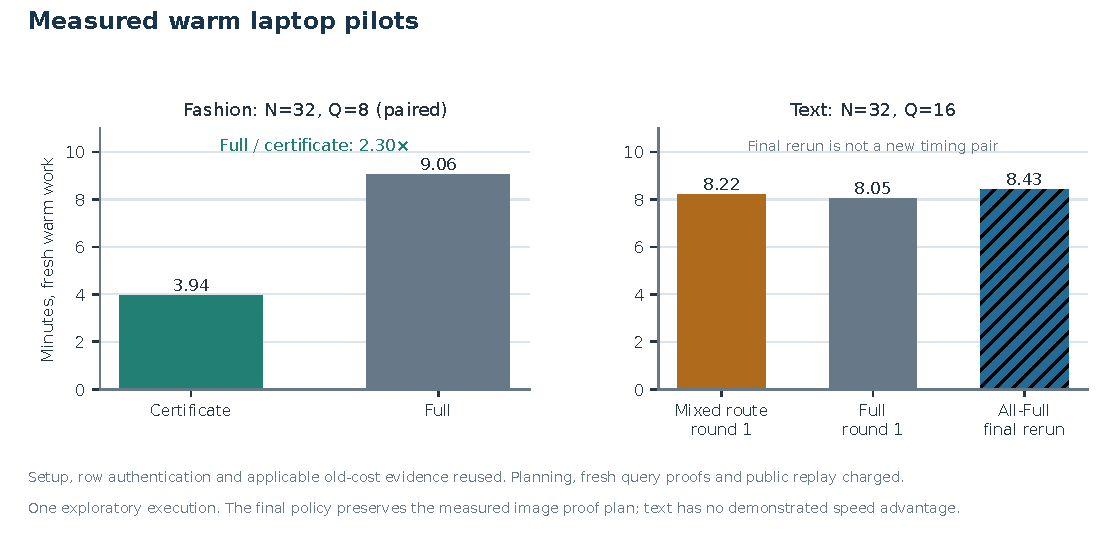
\includegraphics[width=.96\textwidth]{paper_results/ccd_pilot_20261029/figures/06_measured_warm_pilots.pdf}
\caption{Completed warm laptop pilots. The eight-request Fashion row is a paired
comparison. On text with sixteen requests, the mixed-route pair and final all-Full rerun are
separate executions; the latter supplies no new paired speed ratio.
Existing setup and applicable old evidence are reused, while request
proofs and replay are newly executed.}
\label{fig:ccd-warm}
\end{figure*}

\paragraph{Answer to RQ2}
Reusable certificates reduce measured work in the retained Fashion regimes,
but preparation and recurring unsuccessful work both matter. A measured
warm advantage at 64 requests supports reuse; it does not determine the first
cold crossing. No measured 1,000-request threshold or universal crossover is
claimed. Longer fixed-contract sequences remain part of the prospective study.

\subsection{RQ3: Catalog Scale and Proof Material}
\label{sec:ccd-rq3}
The newer Fashion cold pilot with $n=128$ closes four of four requests in 12.467
minutes, compared with 22.838 for Full and 15.525 for the adapter. Peak
process-tree RSS is about 1.269~GiB for the certificate, 1.756~GiB for Full,
and 2.393~GiB for the adapter. The PCA attempt was stopped by a Windows
host-memory notification and is incomplete. That event is not evidence of
an intrinsic PCA memory limit or a completed comparative win.

The archived 1,024-row control demonstrates an additional completed proof
scale, but differs in fit and request workload. It cannot be connected to
the new $n=32/128$ rows as a controlled asymptotic runtime curve. Larger native
catalogs likewise do not establish proof-generation scalability.

Proof storage also depends on which evidence is counted. For the warm
eight-request Fashion cost-aware comparison, fresh request proof bytes total 5,488 for
the certificate and 6,272 for Full. Including reused row/reference proofs
gives 11,760 and 7,056 bytes, respectively. The complete certificate bundle
therefore has more proof bytes despite fewer fresh request bytes. Parameters,
verification keys, proving keys and public metadata are additional material.
The larger Halo2 proof footprint reflects a backend-level system difference
and is not isolated evidence for the compact representation.

\paragraph{Answer to RQ3}
Completed cases show useful time and memory trade-offs, together with added
authentication material. They do not yet provide a systematic common-fit
scaling curve. Such a curve requires matched catalog sizes, request counts,
resource limits and complete comparator measurements.

\subsection{RQ4: Difficult Requests and Cost-Aware Scheduling}
\label{sec:ccd-rq4}
\subsubsection{Avoiding unsuccessful proof work}
The sixteen-request text diagnosis motivates the scheduling variant summarized in
Figure~\ref{fig:ccd-routing}. The native planner computes the same integer
envelope and simulates at most 16 width-ordered exact corrections from the
prover's rows. If the predicted compact plan is inconclusive or too costly,
it selects exact Full before generating compact query proofs. All requests
remain in the public task and every selected answer requires actual proofs.

\begin{figure*}[tbp]
\centering
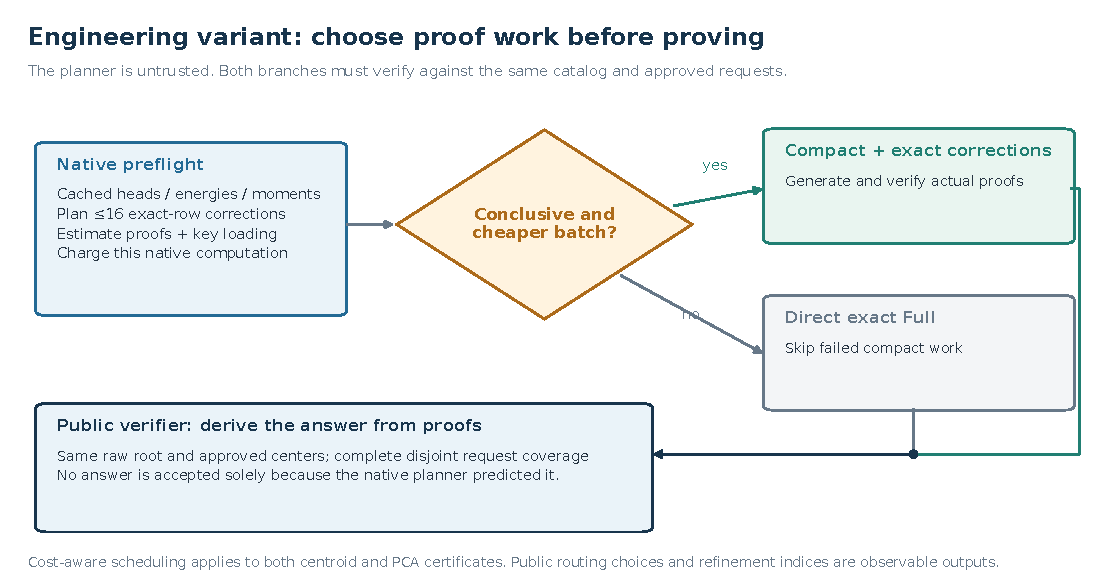
\includegraphics[width=.96\textwidth]{paper_results/ccd_pilot_20261029/figures/05_cost_aware_variant.pdf}
\caption{Cost-aware scheduling variant evaluated after the base protocol.
Native calculations select proof work; they are not verifier evidence.
Complete disjoint request coverage, approved centers and common raw-catalog
pins are checked when merging compact and exact Full branches.}
\label{fig:ccd-routing}
\end{figure*}

The first sixteen-request text policy sends three requests to the certificate and thirteen
directly to Full, eliminating all correction proofs. It nevertheless takes
8.221 minutes versus 8.049 for Full, a 2.15\% slowdown in that execution.
Loading the additional proof-system state consumes much of the predicted
per-request saving. This negative result motivates a batch activation check
that includes certificate/refinement key loading and a saving margin.

The final policy sends all sixteen text requests directly to Full. Its new
warm execution takes 8.427 minutes, including 1.925 seconds of native
planning. There is no newly paired Full reference for this rerun, so its
difference from the earlier Full total is not a speedup or regression
estimate. The same final policy preserves every route in the eight-request Fashion plan and
correction index in the measured image proof plan; image proofs were not
regenerated after this policy-only change. PCA and the adapter were not
retimed in that seed-521 scheduling follow-up. The separate later
seed-557 gate newly measures equally optimized PCA and centroid routes,
with a fresh shared Full comparator.

\subsubsection{Verification and reference lifetime}
Ten native/coverage tests pass for the final scheduling implementation.
A fresh small cryptographic test rejects fifteen substitutions, including
missing or duplicate requests, altered centers or roots, changed keys,
damaged proofs and false costs. All 24 first-round responses and sixteen
repeated final text responses agree with independently recomputed exact
changes. The final text run contains 64 new changing-request proofs; its
reference evidence is retained and reverified. These checks test the
implemented composition rather than proving a general security theorem.

The reuse contract also limits the useful horizon. Installing a different
$C^0$, changing $X$ or replacing the basis invalidates affected authenticated
state. New preprocessing, and any setup required by changed model/circuit
pins, must be charged. A long release batch against one frozen reference
can therefore have a different cost from sequential deployment after every
accepted proposal. No complete end-to-end reference-reset sequence is
measured by the new pilots.

\paragraph{Answer to RQ4}
Preflight can avoid expensive unsuccessful correction paths, but its own
native work and proof-state loading remain costs. The final text policy
deliberately selects Full and demonstrates no compact-path speed benefit.
The main advantage is conditional on informative bounds, affordable proof
work and a sufficiently long valid reference episode.

\subsection{Later Matched Gate against Paper-Derived Baselines}
\label{sec:latest-gate}
\subsubsection{Quality across independently fitted configurations}
Table~\ref{tab:latest-native} pools the three later fits on 128-record
catalogs. Centroid label agreement is 99.80\% on Fashion, 93.49\% on text
and 99.45\% on HAR. It exceeds the tested raw sign/sparse sketches and
one-bit RaBitQ estimates, while PCA remains close: 99.84\%, 92.55\% and
99.51\%, respectively. This does not establish the best possible accuracy
of the full published systems or an advantage in ground-truth class accuracy.
\begin{table*}[tbp]
\centering
\small
\caption{Paper-derived numerical controls on 128 records. Each source pools eight fixed requests from each of three exploratory fits. A is nearest-center label agreement and B is balanced estimated cost-change sign agreement, in percent. These are different tasks; neither is class-label accuracy. Coresets do not predict unsampled labels (--). None of the raw numerical controls supplies a cryptographic certificate.}
\label{tab:latest-native}
\begin{adjustbox}{max width=\textwidth}
\begin{tabular*}{.98\textwidth}{@{\extracolsep{\fill}}lrrrrrr@{}}
\toprule
Method & Fashion A & Fashion B & Text A & Text B & HAR A & HAR B\\
\midrule
Centroid & 99.80 & 100.00 & 93.49 & 50.00 & 99.45 & 80.00\\
PCA & 99.84 & 100.00 & 92.55 & 50.00 & 99.51 & 80.00\\
Sign RP & 92.84 & 100.00 & 68.68 & 66.67 & 93.33 & 67.37\\
Sparse RP & 92.61 & 47.83 & 70.67 & 90.48 & 92.58 & 87.37\\
RaBitQ & 98.50 & 100.00 & 89.32 & 90.48 & 98.44 & 97.37\\
Lightweight32 & -- & 93.48 & -- & 97.62 & -- & 94.74\\
Uniform32 & -- & 100.00 & -- & 100.00 & -- & 62.11\\
\bottomrule
\end{tabular*}
\end{adjustbox}
\end{table*}


Label agreement and aggregate decision estimation can rank methods
differently. On text, 21 of 24 true changes worsen the objective and three
improve it. The centroid/PCA point predictors achieve 87.50\% overall
estimated-sign agreement, equal to always predicting worsening, and
50.00\% balanced agreement. Lightweight32 reaches 97.62\% balanced
agreement; RaBitQ reaches 90.48\%. These useful estimates have different
assurance contracts from an authenticated deterministic decision.

Centroid and PCA both resolve every Fashion and HAR request after at most
16 numerical row corrections, but only 12.50\% of text requests
(Table~\ref{tab:latest-coverage}). Every retained deterministic interval
contains the independently computed exact change, with no wrong certified
labels. The sign/sparse wrappers have much weaker Fashion/HAR coverage;
their nonorthogonal sketches can retain useful raw distance estimates
while leaving large residual norms for this deterministic envelope.
\begin{table*}[tbp]
\centering
\small
\caption{Deterministic numerical decision coverage (percent), before/after at most 16 row corrections, on the same three-fit 128-record cohorts. Every retained deterministic interval contains the exact integer change. The random-projection rows attach our interval relation; poor wrapper coverage is not a failure of the original randomized approximation theorems. These are native bound checks, not proof timings.}
\label{tab:latest-coverage}
\begin{adjustbox}{max width=\textwidth}
\begin{tabular*}{.98\textwidth}{@{\extracolsep{\fill}}lrrrrrr@{}}
\toprule
Basis in our relation & Fashion base & Refined & Text base & Refined & HAR base & Refined\\
\midrule
Centroid & 95.83 & 100.00 & 12.50 & 12.50 & 87.50 & 100.00\\
PCA & 95.83 & 100.00 & 12.50 & 12.50 & 87.50 & 100.00\\
Sign RP + wrapper & 4.17 & 4.17 & 12.50 & 12.50 & 16.67 & 16.67\\
Sparse RP + wrapper & 4.17 & 4.17 & 12.50 & 12.50 & 16.67 & 16.67\\
\bottomrule
\end{tabular*}
\end{adjustbox}
\end{table*}


The RaBitQ statistical intervals resolve 8.33\% of Fashion, 0\% of text
and 12.50\% of HAR requests at $n=128$. No wrong statistical decision or
interval failure is observed among the 144 recorded requests across both
catalog sizes. Observed success is not a deterministic or cryptographic
guarantee, and the finite-query analysis does not cover adaptively chosen
future queries. Appendix~\ref{app:latest-runtime} reports recurring native
times: the raw estimates are generally cheaper than the conservative
integer predictor/bound implementation, and those milliseconds are not
ZK proving times.

\subsubsection{Cold proof work with all fallback charged}
Table~\ref{tab:latest-cold} retains every request in the later matched
32-record proof cohort. Fashion takes 6.690 minutes with centroid, 6.699
with PCA and 7.870 with Full. The small centroid/PCA difference does not
establish a speed ranking. Both random-projection wrappers require one
Full fallback and exceed 14 minutes. The ZKML primitive adapter takes
3.957 minutes and is faster in this cold cohort.
\begin{table*}[tbp]
\centering
\small
\caption{New matched cold proof cohort: 32 records, four requests, seed557, one timing execution. Minutes include enclosing invocation walls, validation, preparation, public replay and all newly generated fallback; certificate totals also charge basis fitting. ZKML diagnostic MockProver work is excluded. Cov. is conclusive compact coverage before Full, or exact responses for Full/ZKML; FB is paid Full fallback. Different backend/output contracts prevent an unqualified proving-system ranking.}
\label{tab:latest-cold}
\begin{adjustbox}{max width=\textwidth}
\begin{tabular*}{.98\textwidth}{@{\extracolsep{\fill}}lrrrrrr@{}}
\toprule
Method & Fashion min. & Cov. & FB & Text min. & Cov. & FB\\
\midrule
Full & 7.870 & 4/4 & 0 & 3.926 & 4/4 & 0\\
Centroid & 6.690 & 4/4 & 0 & 11.046 & 1/4 & 3\\
PCA & 6.699 & 4/4 & 0 & 11.014 & 1/4 & 3\\
Sign RP + wrapper & 14.085 & 3/4 & 1 & 12.634 & 0/4 & 4\\
Sparse RP + wrapper & 14.017 & 3/4 & 1 & 11.875 & 0/4 & 4\\
ZKML adapter & 3.957 & 4/4 & 0 & 2.290 & 4/4 & 0\\
\bottomrule
\end{tabular*}
\end{adjustbox}
\end{table*}


On text, centroid/PCA resolve only one of four requests before fallback
and take 11.046/11.014 minutes, against 3.926 for Full and 2.290 for the
adapter. The sign/sparse wrappers resolve none before fallback. Every
selected exact fallback is newly generated and charged. All completed
public verification and independent integer checks pass; this establishes
correct answers for the recorded workload, not favorable compact economics.

\subsubsection{Equal cost-aware scheduling and reuse}
Table~\ref{tab:latest-warm} applies the same existing policy to all four
bases. On Fashion, centroid takes 2.124 minutes against 4.730 for warm
Full, a ratio of 2.227; PCA takes 2.068 minutes. Both use compact proofs
for every request. The sign/sparse wrappers use three compact requests
and one direct Full request, taking 3.597/3.661 minutes. No current-basis
advantage over equally optimized PCA is established by this execution.
\begin{table*}[tbp]
\centering
\small
\caption{Equal-routing warm follow-up on the same 32-record, four-request cohort. The existing calibration and ten-percent activation margin apply to every basis. Setup, authenticated rows and applicable old evidence are reused equally; fresh request proofs, key loads, whole-batch native planning and public replay are charged. One fresh Full comparator is shared per dataset, not counted as four repetitions. Times are phase-wall minutes, excluding export/copy and independent numerical oracle checks.}
\label{tab:latest-warm}
\begin{adjustbox}{max width=\textwidth}
\begin{tabular*}{.98\textwidth}{@{\extracolsep{\fill}}llrrrrr@{}}
\toprule
Data & Basis/policy & Compact & Full & Service min. & Full min. & Ratio\\
\midrule
Fashion & Centroid & 4 & 0 & 2.124 & 4.730 & 2.227\\
Fashion & PCA & 4 & 0 & 2.068 & 4.730 & 2.287\\
Fashion & Sign RP + wrapper & 3 & 1 & 3.597 & 4.730 & 1.315\\
Fashion & Sparse RP + wrapper & 3 & 1 & 3.661 & 4.730 & 1.292\\
Text & Centroid & 0 & 4 & 2.276 & 2.276 & 1.000\\
Text & PCA & 0 & 4 & 2.282 & 2.276 & 0.998\\
Text & Sign RP + wrapper & 0 & 4 & 2.241 & 2.276 & 1.016\\
Text & Sparse RP + wrapper & 0 & 4 & 2.283 & 2.276 & 0.997\\
\bottomrule
\end{tabular*}
\end{adjustbox}
\end{table*}


On text, every representation routes every request directly to Full.
The centroid service and shared Full comparator both take approximately
2.276 minutes. Small timing differences among the all-Full routes are
single-execution variation, not evidence of a geometric benefit. These
warm totals and the cold totals have different timing boundaries and
cannot be combined into a newly measured cold crossover.

The later gate therefore extends comparative breadth and checks that
scheduling is applied equally, while retaining the same main conclusions:
verified reuse is useful in the measured image regime, PCA is competitive,
and difficult text provides no compact-path speed benefit. Three fits
strengthen numerical breadth; proof replication and scale remain limited.


